\chapter{Implementation}\label{chapter_implementation}
\acresetall

This chapter goes into depth on how the design from the previous chapter is
implemented into the BATMAN protocol. The layout of this chapter is a
chronological order from the point of view of the programmer. The source code
can be found in Appendix \ref{chapter_source_code}.


\section{Classes}

\subsection{Authentication Module}
Almost all functionality added to BATMAN is within the borders of this class.
Some code however, had to be added elsewhere in order to call the \ac{AM}
functions, or to use information from \ac{AM}. This segregation is primarily
done in order to separate original BATMAN functions from new authentication
functions.

The first thing to notice about the \ac{AM} is that it runs in its own thread,
so all authentication mechanisms run concurrent to regular BATMAN routing
operations. This separation was necessary in order to have BATMAN behave
normally during authentication of a node, so a large network should not suffer
if an important node (position) is 'hung up' in authentication.

\subsection{Batman and Schedule Classes}
These were the only classes of the original BATMAN code that had to be modified.
The Batman class handles most of the logic when receiving an \ac{OGM} so this is
where a check has been added to see if a node is known. If it is not, a thread
in the \ac{AM} is initialized in order to try to authenticate with the other
node, and then goes on to disregard the handling of that packet further, as to
deny it being copied into the routing table by BATMAN. The \ac{OGM} packet
format has also been slightly altered as to include an extra field for
authentication purposes. This field will be used to include the signature offset
of the node broadcasting or forwarding the \ac{OGM}.

In the Schedule class the signature offset, or the authentication token as
described in the next section, was added at the end of the extended \ac{OGM}. If
there is no authentication token or signature available, it will add a zero
value, indicating the node is not authenticated with any network.

\begin{figure}[h]
	\centering
	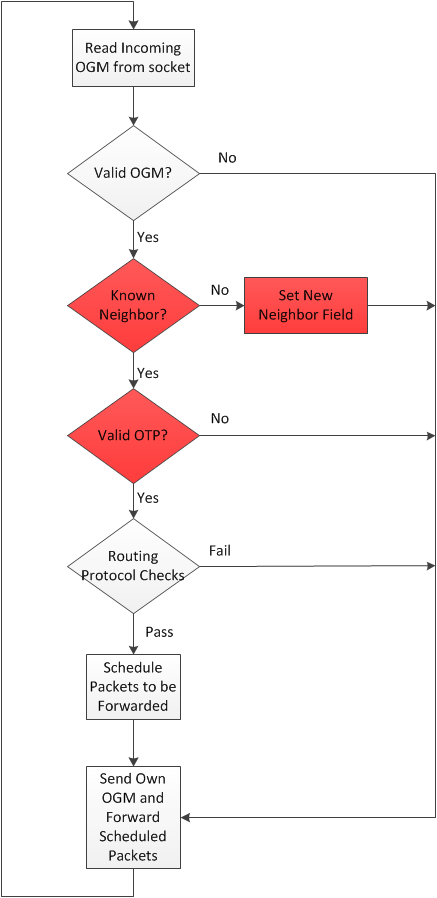
\includegraphics[totalheight=1\textheight]{images/batman_if_statements.png}
	\caption{IF-Statements in the Batman Class}
	\label{fig:batman_if_statements}
\end{figure}

\section{First Phase}
The first phase of the implementation started with looking through the whole
source code of BATMAN in order to get an understanding of where and how changes
had to be made. The batman class has a nice setup where it goes through many
different checks (if-statements) on a received \ac{OGM} to determine wheter it
should be added to the routing table, if information about the node should be
modified, or if the node should be dropped for one of several reasons. These
checks are shown in Figure \ref{fig:batman_if_statements}.

This first phase does not use any cryptographic functions, and will only be used
as a ``framework'' for handling the sent messages and function calls, so adding
actual secure methods later will become separated from the problems of altering
the BATMAN source code.

Throughout all of these checks, there is a label it can jump to if any check
fails, called 'send\_packets'. That is, it is a label in the received packet is
disregarded and the program goes on to schedule its own and and forward other
scheduled \acp{OGM}. In Figure \ref{fig:batman_if_statements} this is shown
with the box at the bottom. This label is very useful because when checking if a
node is already authenticated, the flow can be altered so that if a node is
unknown the program can jump to this label and disregard the handling of the
received \ac{OGM} after initializing a new authentication thread in \ac{AM}.
This part is shown with the highlighted red in the same figure.

In this first phase, a method called 'authenticate\_init' in the \ac{AM} class
is called when an \ac{OGM} is received from an unknown source. This method
copies information about the node such as its IP-address to a local variable
before it initiates a new authentication thread to handle the authentication
phase. The original thread jumps back to the batman class and jumps to the
'send\_packets' label. Until the authentication thread is completed, no new
packets from unknown sources will be handled.

In the authentication thread the first thing that needs to be done is to
determine which node is, or will become, the master node. Assuming both nodes
are already authenticated in the network, which means they both have no
signature offset value set in their \acp{OGM}, a very simple master node choice
is made based on the address value. Whichever of the two nodes have the larger
IP address value is assigned the master role. When authenticating with new nodes
after this point, an authenticated node will disregard unknown nodes
completely, and only the new node and the master node will initiate
the authentication handshake, in which the new node will recognize that the
master node is already authenticated, and therefore the master node, by looking
at the non-zero authentication signature-offset.

Next, the master node will send a pseudo-random challenge value (one-byte
unsigned integer) in a challenge packet. It is important to mention once
again that these packets are meant as a framework, and that the challenges in
the final version will both be much larger in size and made with a
cryptographic function. The challenge packet is defined with an \ac{AM}-header
(ID and payload type) and its payload type which is the one-byte unsigned
integer value of the challenge. This packet, and all following are addressed
directly to each other, and they are not broadcasted through the whole network
such as \acp{OGM}.

The recipient of the challenge will respond with a challenge-response packet
which contains the response value, which is just a value generated as a simple
function of the received challenge value, and a new challenge value for the
master node. Once again, the response value will be created using
cryptographic functions in the final version. This packet is similar to the
challenge packet, only it contains one more field - i.e. for the response value.

The master node will try to verify the response value received in
challenge-response packet and send a new response value to the received
challenge in a new response-packet. This packet, in addition to the response
value, also contains an authentication value, which will be used by all
``authenticated'' nodes as the signature offset during this first phase of the
programming. It should be noted that this is not in any way a secure
authentication, because the authentication handshake contains no cryptographic
functions and does not use any cryptographic keys of any sort, and because
anyone sniffing the network can pick up the authentication value to be used.

If the recipient of the response-packet accepts the response value, it will now
copy the authentication token and use this in its \ac{OGM} later on, and
recognize itself as an authenticated node. That means, as stated earlier, that
it will now totally disregard any recevied \acp{OGM} for which it does not
recognize the signature offset, or authentication value if you will.

TODO: Split into sections and add figures, maybe a MSC to depict the handshake
message flow\ldots

\section{\acf{PC}}

\subsection{Creating a Public Key Pair}

\subsection{Creating the \ac{PC} with the Public Key Pair}

\subsection{\ac{SP} Signing the Unsigned \ac{PC}}

\subsection{Validate the signed \ac{PC1}}

\subsection{Creating a Signature with \ac{PC} (0 and 1)}